\documentclass[a4paper,11pt, openany]{book} %Remove draft option to hide ToDos

\include{header}
\tolerance=200

\settitle{Extending and Automating Iris~Proof~Mode with Ltac2}
\setauthor{Bohdan Liesnikov}
\supervisor{Prof. Dr. Derek Dreyer}
\advisor{Dr. Robbert Krebbers}
\reviewerOne{Prof. Dr. Derek Dreyer}
\reviewerTwo{Dr. Robbert Krebbers, Radbound University Nijmegen, The Netherlands}
\university{Saarland University}
\faculty{Faculty of Mathematics and Computer Science}
\thesistype{Master's }
\subdate{30}{November}{2020}
\city{Delft, The Netherlands}
\setBaseUrl{{https://liesnikov.gitlab.io/masters/coq/}}

\DeclareTextFontCommand{\emph}{\bfseries}


\pagenumbering{roman}

\setlength{\headheight}{15pt}

\pagestyle{fancy}
\renewcommand{\chaptermark}[1]{ \markboth{#1}{} }
%\renewcommand{\sectionmark}[1]{ \markright{#1}{} }

\fancyhf{}
\fancyhead[LE,RO]{\thepage}
\fancyhead[RE]{\textit{ \nouppercase{\leftmark}} }
\fancyhead[LO]{\textit{ \nouppercase{\rightmark}} }

\fancypagestyle{plain}{
	\fancyhf{}
	\renewcommand{\headrulewidth}{0pt}
	\renewcommand{\footrulewidth}{0pt}
}

%\makeglossaries

\begin{document}

\renewcommand\cite{\citep}

\thispagestyle{empty}

\maketitlepage

\statementpage

\electronicpage

\chapter*{Abstract}
\addcontentsline{toc}{chapter}{\numberline{}Abstract}
In this thesis, we use a new experimental tactic language -- Ltac2 to reimplement part of the complex system of which provides tactics for separation logic, as originally presented by MoSeL.
Using this new implementation as a platform for new feature development, we adapt the solution for ``resource distribution'' problem from the work by Harland and Pym to MoSeL entailments, in particular, we adapt old tactics to support postponed decisions about the distribution and and provide a completely new one for introduction of separating conjunction \coqe{iSplit}.
Utilizing Ltac2's notation mechanisms, we also implement a separation-logic alternative for \coqe{match goal}, which incorporates both multiple contexts from MoSeL proof mode and the new proof mode with postponed resource distribution decisions.
Finally, we consolidate the new implemented features to implement a simple solver for separation logic.
In the process we also evaluate Ltac2, reflect on our experiences with development and suggest possible directions for future development of the language.

%%% Local Variables:
%%% TeX-master: "thesis"
%%% End:


\newpage

\chapter*{Acknowledgements}
I would like to thank Prof. Dreyer for suggesting this topic and being my supervisor for the thesis.
However, he did much more than this, he supported and mentored me all the way through my Master's studies and I am extremely grateful for that.

I would also like to thank Dr. Krebbers for providing constant feedback and guiding me through the process of development of the thesis.
I'm also indebted to Michael Sammler, Ike Mudler and Coq community at large for fruitful discussions and helpful suggestions.

Finally, but perhaps, most importantly, I would like to thank my family and friends.
You know who you are.
I wouldn't make it even half-way without your support and love.
Without the time we spent together.
Without your help.
Thank you.


%%% Local Variables:
%%% TeX-master: "thesis"
%%% End:

\addtocontents{toc}{\vspace{5mm}}

\tableofcontents

\listoftodos

\clearpage
\pagenumbering{arabic}

\chapter{Introduction}

This thesis is about interactive proof development for separation logic.
In the introductory chapter we give an overview for history of developments of mechanized tools for separation logic, highlight some of the gaps of existing developments and list our contributions to the subject.

\section{Separation logic and mechanization}
\label{sec:separation-logic-mechanization}

Separation logic (SL) was introduced by \citet{reynoldsSeparationLogicLogic2002} and
\citet{ohearnLocalReasoningPrograms2001} as a solution to problems with reasoning about mutable data structures.
It proved to be widely successful \cite{ohearnSeparationLogic2019} and served as a basis for multiple other developments of logics used for reasoning about programs, the most influential of them, perhaps, being Concurrent Separation Logic (CSL) by \citet{ohearnResourcesConcurrencyLocal2007}.

In the last decade there were multiple new advanced logics developed that are both higher-order and based on Concurrency Separation Logic, like one that serves as a foundation for Verified Software Toolchain by \citet{appelProgramLogicsCertified2014} or Iris \cite{jungIrisGroundModular2018}, which was used to establish formal foundations of Rust programming language \cite{jungRustBeltSecuringFoundations2018}.

Separation logic also gave rise to multiple mechanized tools.
Initial applications of separation logic to mechanized developments were concentrating on mostly automatic proofs, like Smallfoot~\cite{berdineSmallfootModularAutomatic2006} or Verifast~\cite{jacobsVeriFastProgramVerifier2008} or Bedrock~\cite{chlipalaMostlyautomatedVerificationLowlevel2011, chlipalaBedrockStructuredProgramming2013}.
With this approach logics have to be restricted in order for automation to be feasible, as on its own even separation logic with a magic wand \((\wand)\) is undecidable \cite{brotherstonUndecidabilityPropositionalSeparation2014}.

However, automatic proofs are not the only possibility and they are not suitable for more expressive variants of SL, which can include advanced connectives, such as modalities and views.
The alternative to automatic verification is tactic-based interactive verification.
There are multiple developments that pursue this idea, usually utilizing existing interactive proof assistants: ``Charge!''~\cite{bengtsonCharge2012},
, VST-Floyd~\cite{caoVSTFloydSeparationLogic2018} for Verified Software Toolchain, MoSeL for Iris \cite{krebbersInteractiveProofsHigherorder2017, krebbersMoSeLGeneralExtensible2018}.
In fact, MoSeL (and its predecessor, IPM -- Iris Proof Mode) turned out to be essential for developments based on Iris \cite{krebbersMoSeLGeneralExtensible2018, jungUnderstandingEvolvingRust2020}: verification of Rust's safety claims \cite{jungRustBeltSecuringFoundations2018, jungStackedBorrowsAliasing2019, dangRustBeltMeetsRelaxed2019}, formalization of Scala's core type system \cite{giarrussoScalaStepbystepSoundness2020}, framework for concurrent reasoning based on message-passing \cite{hinrichsenActrisSessiontypeBased2019} and many others.

VST-Floyd~\cite{caoVSTFloydSeparationLogic2018} and MoSeL \cite{krebbersMoSeLGeneralExtensible2018} are two most recent major pieces of work in the direction of tactic-based interactive verification.
Both of them provide support for automation, though differ significantly in approaches.
VST-Floyd follows the idea of normal form for goals, which was also used in \cite{bengtsonCharge2012} and is focused tactics for one specific logic and forward-style reasoning approach.
MoSeL, on the other hand, doesn't try to normalize goals and places emphasis on genericity of the logic: it builds on the interface of Modal Bunched Implications (MoBI) logic, which allows user to apply it in any logic that instantiates the interface.

\section{Problems and approaches}
\label{sec:problems-approaches-intro}

While MoSeL achieved a lot, there still are some issues with the current state of the tool.
We now describe the problems and our approach to solving them in this thesis.

\subsection{Ltac1 issues}
\label{sec:ltac1-issues}
Ltac was the first tactic language for Coq that allowed extensive automation and it served Coq well, being called ``major ingredient of the success'' of Coq \cite{pedrotLtac2TacticalWarfare2019}.
Unfortunately, it has outgrown its original purpose and is now known to be a problematic for developments of non-trivial complexity.
It has badly defined semantics, such that even maintainers don't understand the order of evaluation \cite{pedrotLtacInternals2016}, it lacks clear distinction between Coq variables and Ltac variables \cite{pedrotLtacInternals2016}, proper exceptions, ability to deal with existential variables and even documentation says that some tactics should be used ``at your own risk'' \cite[Section~3.3.1]{thecoqdevelopmentteamCoqProofAssistant2020}.
MoSeL also relies on Ltac to a great extent and this used to be a handicap for its development and maintenance, because of the fragility of larger programs written in Ltac.

Fortunately, since the problem with Ltac are well-known, many other languages appeared to substitute it \cite{malechaExtensibleEfficientAutomation2016, zilianiMtacMonadTyped2013, kaiserMtac2TypedTactics2018a, tassiElpiExtensionLanguage2018}.
There is also a new experimental tactic language that aims to be a direct successor of Ltac, trying to stay as close as possible to Ltac, while maintaining sane semantics: Ltac2 \cite{pedrotLtac2TacticalWarfare2019}.

We rewrite Ltac parts of MoSeL to Ltac2, trying to improve the implementation where possible and use this new version of MoSeL to develop new features.

\subsection{\coqe{iSplit} tactic}
\label{sec:isplit-tactic}

One of the main problems with incorporating backwards-style proofs to separation logic is the introduction rule for a new connective -- ``separating conjunction''.
\[\infer{\Gamma_1, \Gamma_2 \vdash \phi_1 \ast \phi_2}
        {\Gamma_1 \vdash \phi_1 &
         \Gamma_2 \vdash \phi_2} \]
The logic is substructural since it lacks contraction rule, so introduction of separating conjunction forces us to distribute hypotheses between two branches of the proof.
However, this creates a problem with bottom-up proof construction, since we frequently don't know which propositions will be needed in which branch until it's finished.

In MoSeL, introduction of separating conjunction corresponds to \coqe{iSplit} tactic (separation logic variant of \coqe{split}).
It requires a user to provide a list of hypotheses that will be attributed to either left (\coqe{iSplitL}) or right (\coqe{iSplitR}) branch, essentially guessing beforehand which hypotheses are going to be used where.

The issue with the rule was first described in a paper by \citet{harlandResourceDistributionBooleanConstraints2003}.
They proposed an amended entailment predicate to solve the problem.
The idea is to postpone the distribution by attaching Boolean flags (\(e_1, e_2\)) that indicate presence of hypotheses and imposing a side-condition that the flags are disjoint.
\[\infer[e_i \oplus \hat{e}_i = \true, i \in \{1,2\}]
        {P, Q \vdash \phi_1 \ast \phi_2}
        {P[e_1], Q[e_2] \vdash \phi_1 &
         P[\hat{e}_1], Q[\hat{e}_2] \vdash \phi_2} \]
We adapt their solution to MoSeL and create a new \coqe{iSplit} tactic, that doesn't require the user to provide such a list.

\subsection{Goal matching}
\label{sec:goal-matching}

One of the very useful tacticals of Ltac was \coqe{match goal}.
It allows a user to match the hypothesis and the goal in the current proof state and has proven to be essential for automation tactics, i.e. it is used in \coqe{naive_solver} from stdpp~\cite{ProjectsIrisStdpp}, one of the first examples in CPDT~\cite{chlipalaCertifiedProgrammingDependent2013} and \coqe{break_match} tactic from StuctTact library~\cite{UwplseStructTact2020}.
\begin{coq}
match goal with
| [H : False |- _] => exfalso; exact H
| [|- True] => exact I
end.
\end{coq}

MoSeL doesn't use Coq contexts and instead stores hypothesis in the goal, which renders the original tactical unfit for it, and Ltac doesn't provide a way to reuse the syntax of goal matching for user-defined tactics.
We develop a new tactic \coqe{iMatch goal} in Ltac2 for reimplemented MoSeL, which aims to be a separation-logic alternative to \coqe{match goal}.
  
\section{Contributions}
\label{sec:contributions}

\begin{itemize}
\item In chapter~\ref{chap:reimplementation_ipm}, we describe reimplementaion of MoSeL in Ltac2, thus contributing one of the first significant applications of the language.
  In the process, we evaluate parts of the language used and suggest possible directions for future development.
\item In chapter~\ref{chap:postponed_splitting}, we develop and adaptation of results by \citet{harlandResourceDistributionBooleanConstraints2003} to MoSeL, as reimplemented in the previous chapter, to introduce a new splitting tactic \coqe{iSplit}.
\item In chapter~\ref{chap:imatch}, we describe a new primitive \coqe{iMatch goal} for tactic language of separation logic, which allows us to match entailments akin to Coq's native \coqe{match goal} construct.
\item Finally, in chapter~\ref{chap:solver} we bring the implemented features together in order to implement a solver for separation logic.
\end{itemize}
We conclude with an overview of related work~\ref{cha:related-work}.

%%% Local Variables:
%%% mode: latex
%%% TeX-master: "thesis"
%%% TeX-parse-self: t
%%% TeX-auto-save: t
%%% reftex-cite-format: natbib
%%% reftex-default-bibliography: ("/home/buzzer/my-dir/ed/uni/saar/prjcts/iris/npm/tex/TacticsProofs.bib")
%%% End:
\chapter{Ltac2}

Ltac2 is a new developing tactic language for Coq Proof assistant.
It comes as a successor to Ltac, which original implementation of Iris Proof Mode relies heavily on.
The need for a new tactic language is well justified, since Ltac was originally 


\section{Semantics of Ltac2}

\begin{itemize}
  \item Links to the new tactic engine as per PMP's post
  \item Derivation of the Ltac2 monad with examples
  \item Implementation of few showcased tactics with Ltac2
\end{itemize}

\section{Standard library for Ltac2 and differences from Ltac1}

\begin{itemize}
  \item Datatypes
  \item Exceptions
  \item Notations
  \item Scopes
\end{itemize}


%%% Local Variables:
%%% TeX-master: "thesis"
%%% End:

\chapter{Reimplementation of IPM in Ltac2}
\label{chap:reimplementation_ipm}

In the previous two chapters we covered both basics of separation logic and one of the tactic languages of Coq -- Ltac2.
This chapter is, to some extent, combining these two parts: we explain details of the implementation of Iris Proof Mode in Coq.

The original implementation of Iris Proof Mode is due to
\citet{krebbersInteractiveProofsHigherorder2017}.
It was later extended to MoSeL \citet{krebbersMoSeLGeneralExtensible2018}, a general framework for modal separation logics in Coq.
This thesis builds on MoSeL and follows its implementation closely.

However, while the original work was done using Ltac1, here we present a translation to Ltac2.

MoSeL itself, as follows from the title of the original paper is framework for separtion logic in Coq, which allows for easier formally verified proofs.
The idea is to embed separation logic in Coq and provide necessary infrastructure for a user to apply their intuitions and skills with tactics.

The structure of the chapter is as follows:
\begin{itemize}
\item First we describe the embedding of logic in Coq and how Iris Proof Mode entailments correspond to the theory.
\item Then we go into the details of the implementation of tactics and proof mode.
\item Finally, we share some experiences from the translation of Ltac1 implementation to Ltac2.
\end{itemize}

\section{Iris Proof Mode from theoretical perspective}
\label{sec:ipm_theory}
There are several options for embedding one (object) logic into another (meta) logic, but among them two most commonly used ones are ``shallow embedding'' and ``deep embedding''.

The first one corresponds to mapping propositions in the object logic directly to their semantics in meta-logic.
I.e. for classical separation logic we would map propositions to predicates over heaps.
This would map separating conjunction \(P * Q\) to \(\lambda \sigma.\,\exists\sigma_1, \sigma_2.\, \left(\sigma = \sigma_1 \uplus \sigma_2\right) \wedge P (\sigma_1) \wedge Q(\sigma_2)\) and separation logic entailment \(P \vdash Q\) to \(\forall \sigma. P \sigma \implies Q \sigma\).

Deep embedding, on the other hand, defines syntax of the object logic in meta-logic explicitly.

And while shallow embedding allows us to re-use re-use meta-logic connectives and binders for some constructions, like implication in the example above or quantifiers, for others we have to make up more involved propositions.

The latter complicates proofs of entailments in the object logic when done within meta-logic.

Instead, MoSeL opts for abstraction of inference rules of the separation logic.
From a user perspective, this gives them both connectives and their inference rules, as well as some properties.

For separating conjunction we get the usual commutativity, associativity and distributivity properties, as well as what MoSeL calls a \textsc{sep-mono} rule:
\[(P_1 \vdash Q_1) \text{ and } (P_2 \vdash Q_2) \,\, \implies \,\, P_1 * P_2 \vdash Q_1 * Q_2\]

However, while this allows axiomatic reasoning in object-logic, it still doesn't support tactics, which Coq users are used to.

In particular, take the following entailment in affine separation logic:
\(P * Q * R \vdash R\).
A user would want to simply apply an ``assumption'' tactic, since relevant resource is clearly in the context and the rest can be discarded, since the logic is affine.

And without tactics, one solution would be convert right side of the entailment to \(\emp * (\emp * R)\) via double application of the property of \emp being neutral element for separating conjunction.
Then use \textsc{sep-mono} rule twice and ``drop'' both \(P\) and \(Q\) on the respective branches of the proofs, since the logic is affine.

We will continue using \coqe{assumption} as our running example in this chapter.

One of the problems that complicates implementation of tactics is that left-hand side of the entailment above doesn't have any structure to it that we could operate on.

To solve this, instead of using arbitrary bunches, MoSeL uses lists of resources and defines new entailment predicate:

\[\entailsOneD Q \defeq \Sep \Pi \vdash Q\]
where \(\SpatD\) is a list of pairs of identifiers and separation logic propositions \(\SpatD \defeq H_1 : P_1, \ldots , H_n : P_n\) and \(\Sep\) is an iterated separating conjunction.

If we substitute the definition of \(\SpatD\) and \(\Sep\), the entailment definition takes the following form.
\[\left( \entailsOne {H_1 : P_1, \ldots , H_n : P_n} Q \right) \defeq
  \left( P_1 * \ldots P_n \vdash Q \right)\]

In fact, the definition is slightly more general, as it incorporates two lists \(\IntuD\) and \(\SpatD\):
\[\entailsD Q\]
Where \(\IntuD\) is also a list of resources, but in the definition of the entailment it gets mapped to iterated non-separating conjunction with \(\intuit\) modality:

 \[\entailsD Q \defeq \intuit \left(\bigwedge \IntuD\right) * \left(\Sep \SpatD\right) \vdash Q\]

This allows us to introduce new derivation rules, that work more like tactics.

\subsection{Rules for regular IPM}
\label{sec:rules-regular-ipm}

Now that we have formalized Iris Proof Mode entailment, we can also translate some tactics from just Coq proof state transformers to derivation rules.
We aren't going to give a complete list of tactics, but just a few to illustrate translation.

Regular introduction rules don't change that much, except now the context has to stay in particular shape.

\begin{itemize}
\item To introduce a magic wand we extend the spatial context with a new resource.
  \[\infer[\textsc{Tac-wand-intro}]
      {\entailsD P \wand Q}
      {\entails {\IntuD} {\SpatD, i : P} {Q} &
       i \text{ is a fresh identifier}}
  \]
  If the resource introduced is intuitionistic, we can put it directly into an intuitionistic context, while stripping away the modality.
  \[\infer[\textsc{Tac-wand-intro-intuit}]
      {\entailsD \intuit P \wand Q}
      {\entails {\IntuD, i : P} {\SpatD} {Q} &
       i \text{ is a fresh identifier}}
  \]
\item The rule for separating conjunction also stays very similar to the original one
  \[\infer[\textsc{Tac-sep-intro}]
      {\entailsD P * Q}
      {\entails {\IntuD} {\SpatD_1} P &
       \entails {\IntuD} {\SpatD_2} Q &
       \SpatD \equiv \SpatD_1 {+\hspace{-0.5em}+} \SpatD_2}
   \]
   \todo{swap for real append operator}
   Where \({+\hspace{-0.5em}+}\) is \coqe{append} operator for lists and \(\equiv\) is list equivalence.

   Note that intuitionistic context doesn't have to be split, since resources in it are duplicable, hence we can access them in both branches of the proof.
\item Before we get to an \coqe{assumption} tactic, let's consider \coqe{exact H}, which closes goals with assumption \coqe{H} from the context.
  The following would be a correct, but not very useful tactic:
  \begin{align*}
      \infer
        {\entailsD P}
        {\SpatD = [H : P]}
    & \hspace{5em}
    & \infer
        {\entails {\IntuD} {[\,]} P}
        {H : P \in \IntuD}
  \end{align*}
  In the first case here there aren't any requirements for the intuitionistic context, since resources in it are affine by definition.
  This doesn't hold for spatial context in general unless the logic we're working is affine.

  However, both of the variants put significant restrictions on spatial context, which can be lifted slightly.
  As noted above, one could create a specialized tactic for affine logic, but instead MoSeL asks for the rest of the context to only contain affine resources, so the tactic becomes:
  \begin{align*}
      \infer%[\textsc{tac-exact-spatial}]
        {\entailsD P}
        {H : P \in \SpatD &
         \SpatD \backslash (H : P) \text{ is affine}}
    & \hspace{5em}
    & \infer%[\textsc{tac-exact-intuitionistic}]
        {\entails {\IntuD} {[\,]} P}
        {H : P \in \IntuD &
         \SpatD \text{ is affine}}
  \end{align*}
  We call a context affine if it only contains affine resources and stick to convention that in affine logic all resources are affine.
\item Generalization of the tactic above to behave more like \coqe{assumption} is trivial -- instead of asking for a specific \(H : P\) to be in the context, we ignore identifiers entirely and the assumption becomes that there is some \(P\) in the context
  \begin{align*}
      \infer%[\textsc{tac-assumption-spatial}]
        {\entailsD P}
        {\exists H. H : P \in \SpatD &
         \SpatD \backslash (H : P) \text{ is affine}}
    & \hspace{5em}
    & \infer%[\textsc{tac-assumption-spatial}]
        {\entails {\IntuD} {[\,]} P}
        {P \in \IntuD &
         \SpatD \text{ is affine}}
  \end{align*}
\end{itemize}

% \begin{itemize}
% \item Start proof
% \item Context maninputation
%   \begin{itemize}
%   \item iRename
%   \item iClear
%   \item iEval
%   \end{itemize}
% \item Assumptions
%   \begin{itemize}
%   \item iExact
%   \item iAssumption
%   \end{itemize}
% \item Intuitionistic/Spatail/Pure transitions
%   \begin{itemize}
%   \item iIntuitionistic
%   \item iSpatial
%   \item iPure
%   \item iEmpIntro
%   \item iPureIntro
%   \end{itemize}
% \item iFrame
% \item Intro of wand/implication
% \item Revert
% \item Specialize and Pose
% \item Apply
% \item Existential
%   \begin{itemize}
%   \item Intro
%   \item Destruct
%   \end{itemize}
% \item Modalities
% \item iDestruct
% \item iIntros
% \item Induction
% \item Löb
% \item Assert
% \item Rewrite
% \end{itemize}

\subsection{Implementation of IPM}
\label{sec:implementation-of-ipm}

Now that we have seen Iris Proof Mode from theoretical perspective, let's turn to Coq implementation.

We start with an overview of components of the implementation and build \coqe{iAssumption} tactic in the end.

\begin{figure}[H]
  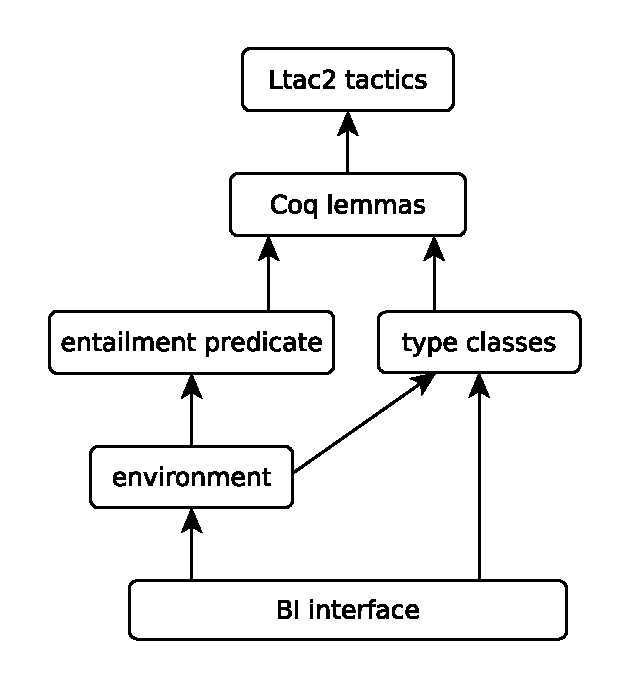
\includegraphics[width=0.5\linewidth]{ipm-diagram}
  \caption{structure of the implementation of IPM}
\end{figure}

The idea is that user instantiates BI interface with their logic and can profit from the existing infrastructure.
Environments, entailment predicates are used to make proofs of ``Coq tactics'' easier and typeclasses allow for more general unification and proof search.
Coq tactics themselves are verified transformations of the goal, the simplest instance being \coqe{tac_ex_falso}.
These transformations are then applied within Ltac2 tactics, which can combine them, use specialized tactics for the subgoals they generate and handle errors.

\subsubsection{BI interface}
\label{subsubsec:bi-interface}

There are five main components, starting with a base interface for BI logic, which we mentioned before and which \citet{krebbersMoSeLGeneralExtensible2018} call MoBI interfaces.

We include it here, with some omissions:
\begin{coq}
Structure bi := Bi {
  bi_car :> Type;
  bi_dist : Dist bi_car;
  bi_emp : bi_car;
  bi_and : bi_car → bi_car → bi_car;
  bi_forall : forall A, (A → bi_car) → bi_car;
  bi_sep : bi_car → bi_car → bi_car;
  bi_wand : bi_car → bi_car → bi_car;
  bi_persistently : bi_car → bi_car;
  bi_pure : Prop → bi_car;
  bi_bi_mixin : BiMixin $\ldots$;
  $\ldots$
}.
\end{coq}

Where \coqe{BiMixin} describes axioms that connectives should satisfy, from associativity of separating conjunction to elimination rule for persistent modality.

With some notation definitons this allows writing and proving BI propositions, only requiring an instance of \coqe{bi}.

\begin{minipage}{\linewidth}
\begin{coq}
Context {PROP : bi}.
Lemma persistently_mono P Q : (P |- Q) → <pers> P |- <pers> Q.
\end{coq}
\end{minipage}

Proving such statement at this point requires applying axioms from \coqe{bi} by hand.

\subsubsection{Environments and entailment predicate}
\label{subsubsec:environment-entailment-pred}

In order to define IPM entailment, we first define contexts.
In general, since most of the tactics only have to deal with one hypothesis from the context or don't even touch existing ones (like \coqe{iIntro}), we use deep embedding to allow easier syntactical transformations.

Environments are defined as association lists with identifiers used as keys and BI propositions as values.

\begin{coq}
Inductive ident :=
  | IAnon : positive -> ident
  | INamed :> string -> ident
Inductive env (A : Type) : Type :=
  | Enil : env A
  | Esnoc : env A -> ident -> A -> env A.
\end{coq}

We also define coercion from \coqe{env} to lists, simply disregarding identifiers.
However, as described above MoSeL entailment predicate includes two context: spatial and intuitionistic, so we define another structure to include both:

\begin{coq}
Record envs (PROP : bi) := Envs {
  env_intuitionistic : env PROP;
  env_spatial : env PROP;
  env_counter : positive (** A counter to generate fresh hypothesis names *)
}.
\end{coq}

Then we can define entailment predicate, which includes not only both contexts, but also a proof that identifiers in each context are unique \coqe{envs_wf $\Delta \urcorner$}.
\begin{coq}
  Definition envs_entails {PROP} ($\Delta$ : envs PROP) (Q : PROP):
  $\ulcorner$ envs_wf $\Delta \urcorner$ /\ $\intuit$ [$\wedge$] env_intuitionistic $\Delta$ * [*] env_spatial $\Delta$ |- Q
\end{coq}

Here \coqe{[*]} is an iterated separating conjunction, defined on lists as folds with respective operation, the same way as it was defined in theoretical presentation.

At this point we can already write some statements in both readable and easy to prove form:
\coqe{Lemma tac_ex_falso Delta Q : envs_entails Delta False → envs_entails Delta Q.}

\subsubsection{Typeclasses}
\label{subsubsec:typeclasses}

Typeclasses serve multiple purposes in MoSeL development, here we are going to describe only couple of simplest instance needed for \coqe{iAssumption}.
The primary idea, however, is to do simple instances of proof search automatically via logic programming.

The first example we are going to look at concerns \coqe{Affine} and \coqe{AffineEnv}.
The former is defined simply as
\begin{coq}
Class Affine {PROP : bi} (Q : PROP) := affine : Q |- emp.
\end{coq}

With instances covering both basic connectives
\begin{coq}
Global Instance emp_affine : Affine emp.
Global Instance and_affine_l P Q : Affine P → Affine (P /\ Q).
Global Instance and_affine_r P Q : Affine Q → Affine (P /\ Q).
Global Instance sep_affine P Q : Affine P → Affine Q → Affine (P * Q).
Global Instance exist_affine {A} (Phi : A → PROP) :
  (forall x, Affine (Phi x)) → Affine (exists x, Phi x).
$\ldots$
\end{coq}

And modalities
\begin{coq}
Global Instance affinely_affine P : Affine (<affine> P).
Global Instance affinely_if_affine p P : Affine P → Affine (<affine>?p P).
Global Instance intuitionistically_if_affine p P : Affine P → Affine ($\intuit$?p P).
\end{coq}

For the environment to be affine we simply require all resources in the context to be affine:
\begin{coq}
Class AffineEnv (Γ : env PROP) := affine_env : Forall Affine Γ.
Global Instance affine_env_nil : AffineEnv Enil.
Global Instance affine_env_snoc Γ i P :
  Affine P → AffineEnv Γ → AffineEnv (Esnoc Γ i P).
\end{coq}

The next example is slightly more advanced and concerns entailment of one proposition with another.
To be more precise, we want to define a typeclass which corresponds to intuitive ``\(P\) is almost the same as \(Q\)''.
\begin{coq}
Class FromAssumption {PROP : bi} (p : bool) (P Q : PROP) :=
  from_assumption : $\intuit$?p P |- Q.
\end{coq}

There are two subclasses of it, providing instances where either the first or the second proposition is treated as an input.
\begin{coq}
Class KnownLFromAssumption {PROP : bi} (p : bool) (P Q : PROP) :=
  knownl_from_assumption :> FromAssumption p P Q.
Class KnownRFromAssumption {PROP : bi} (p : bool) (P Q : PROP) :=
  knownr_from_assumption :> FromAssumption p P Q.
\end{coq}

The difference between their instances is that for \coqe{KnownLFromAssumption} we ``match'' input \(P\) with structural rules and Q is an output and vice-versa for \coqe{KnownRFromAssumption}.
This allows for more effective search, but for our purposes is a mere technicality, so we will only consider \coqe{KnownRFromAssumption}.

While the simplest instance of this is just identity \coqe{P |- P}, there are several more defined in MoSeL, which generalize it.
For example, given that we can prove \(\intuit P \vdash Q\), we can also prove \(\intuit P \vdash \affine Q\) and  \(\intuit P \vdash \intuit Q\).
\begin{coq}
Global Instance from_assumption_affinely_r P Q :
  FromAssumption true P Q → KnownRFromAssumption true P ($\affine$ Q).
Global Instance from_assumption_intuitionistically_r P Q :
  FromAssumption true P Q → KnownRFromAssumption true P ($\intuit$ Q).
\end{coq}

\subsubsection{Coq tactics}
\label{sec:coq-tactics}

As mentioned above, Coq tactics are verified goal transformations, which can be as simple as rules for \coqe{exfalso}, but also more advanced, like the one for \coqe{iAssumption}.

\begin{coq}
Lemma tac_assumption Delta i p P Q :
  envs_lookup i Delta = Some (p,P) →
  FromAssumption p P Q →
  (let Delta' := envs_delete true i p Delta in
   if env_spatial_is_nil Delta' then TCTrue
   else TCOr (Absorbing Q) (AffineEnv (env_spatial Delta'))) →
  envs_entails Delta Q.
\end{coq}

\coqe{envs_lookup} returns a boolean for the context it found identifier \coqe{i} within and proposition \(P\) that was associated with it.

Second assumption guarantees that \(P\) entails \(Q\) and the last one checks that we can disregard the rest of the spatial resrouces in \(\Delta\).
If spatial context is empty, there is nothing to disregard, but otherwise either the whole environment must be affine, or the goal should be able to absorb them:
\(\forall Q, P * Q \vdash \absorb P\).

No other subgoals are generated, since this is the leaf of a derivation.

\subsubsection{Ltac2 tactics}
\label{sec:ltac2-tactics}

The final piece of the puzzle is Ltac2 layer.
While Coq tactics provide verified goal transformations, they require several inputs.
The balance between what should go into a Coq statement and Ltac2 function is about how easy is it to verify something.

Turning again to \coqe{iAssumption}, the idea is that a user doesn't provide explicit identifier of the resource they have in mind, instead tactic is supposed to find it on its own.

Simply asserting existence of such identifier in a Coq lemma doesn't solve anything, since ultimately we have to apply this transformation to the goal and user will have to provide it.

Instead, we go through all elements of the environment and try to apply Coq lemma.
And since there are two contexts to go through, we factor out recursion into a \coqe{find} function, which takes a Boolean flag \coqe{p} to tell apart spatial and intuitionistic context, context \coqe{g} and proposition \coqe{q}.
We then apply \coqe{tac_assumption} defined above and discharge the goals with specialized tactics.
The first goal (\coqe{envs_lookup i Delta = Some (p,P)}) is computational, so \coqe{pm_reflexivity} performs the computation and tries \coqe{reflexivity} tactic.
The other two concern type classes, so we use a wrapper around \coqe{typeclasses eauto} to solve them.

\begin{coq}
  Ltac2 i_assumption () :=
  let rec find (p : coq_bool) (g : ipm_env) (q : ipm_prop) :=
      lazy_match! g with
      | Esnoc ?gg ?j ?pp =>
        first [ refine '(tac_assumption _ \$j \$p \$pp _ _ _ _) >
                [ pm_reflexivity () | i_solve_tc () | pm_reduce (); i_solve_tc ()]
              | find p gg q]
      end
  in
  lazy_match! goal with
  | [|- envs_entails (Envs ?gp ?gs _) ?q] =>
     first [ find '(true) gp q
           | find '(false) gs q
           | i_assumption_coq ()
           | Control.zero (Iriception (os "no assumption matching " ++ oc q ++ os " was found"))]
end.
\end{coq}

The only part which wasn't described so far is \coqe{i_assumption_coq ()}.
This is an example of tactics composition -- \coqe{i_assumption_coq} is essentially applying a different lemma from \coqe{tac_assumption}, which tries to find an assumption of shape \(\vdash Q\) in the Coq context instead of IPM context.

This example also showcases some error handling in the last case, if none of the attempts before succeeded.

\section{Examples of Ltac2 features are/can be used}

While translating implementation from Ltac1 to Ltac2, we encountered several points where Ltac2 was particularly useful.

\paragraph{Fix arities from original IPM}

In the original implementation there aren't tactics of arbitrary arity.
Instead, due to Ltac limitations, developers were forced to define several variants of tactics, each with fixed arity.

\begin{coq}
Tactic Notation "iExists" uconstr(x1) "," uconstr(x2) :=
  iExists x1; iExists x2.
Tactic Notation "iExists" uconstr(x1) "," uconstr(x2) "," uconstr(x3) :=
  iExists x1; iExists x2, x3.
Tactic Notation "iExists" uconstr(x1) "," uconstr(x2) "," uconstr(x3) ","
    uconstr(x4) :=
  iExists x1; iExists x2, x3, x4.
\end{coq}

With Ltac2 we can use scopes for lists, which allow arbitrary arities.
The example above would look as follows:

\begin{coq}
  Ltac2 Notation "iExists" lc(list1(thunk(seq(constr, with_bindings)), ",")) :=
  i_exists lc.
\end{coq}

Where \coqe{i_exists} iterates over the list and applies \coqe{iExists} to each element.

\paragraph{Error messages}

Another pain point of Ltac development is lack of proper error handling.

With Ltac2 there two features that help -- we can define our own custom error classes and there is a proper error handling mechanism, which allows us to match on the error thrown.

As with the \coqe{i_assumption} above, there are multiple instances of nesting tactics within each other.
One way to improve error message thrown by iAssumption would be to catch potential error thrown by \coqe{i_assumption_coq} and append it to the error message produced in \coqe{i_assumption}, so that user can see why the tactic failed.


\begin{itemize}
\item \todo{there's more to do here} I haven't touched Typeclass search yet and not sure there's much I can do in general
\end{itemize}

\section{Missing from Ltac2: notations for intropatterns, user-defined scopes?}

However, there are several very desirable missing features from Ltac2, which impacted potential improvements.

\paragraph{User-defined scopes}

Perhaps, one of the most prominent missing elements from our implementation is intropatterns, since the proper way to define them with Ltac2 would be to extend datatype for intropattern with IPM-specific symbols and then parse it with a custom scope.

However, the latter isn't currently possible without extending OCaml implementation of Ltac2, either via forking Coq or using an Ocaml plugin that modifies Ltac2 grammar.

\paragraph{User-defined pretty-printing}
Another missing feature would be lack of user-defined printing rules.
At the moment this mostly impacts error printing, since we have to rely on the Ltac2 pretty-printer, as notations are parsing-only.

\paragraph{notypeclasses refine}

\paragraph{Interop between Ltac1 and Ltac2?}
\todo{more here}
i.e.\ iris indent-string has to go through the goal to get the result from one to another.

%%% Local Variables:
%%% mode: latex
%%% TeX-master: "thesis"
%%% TeX-parse-self: t
%%% TeX-auto-save: t
%%% reftex-cite-format: natbib
%%% reftex-default-bibliography: ("/home/buzzer/my-dir/ed/uni/saar/prjcts/iris/npm/tex/TacticsProofs.bib")
%%% End:
\chapter{Reimplementing MoSeL in Ltac2}
\label{chap:ltac2-tactics-mosel}

In this chapter we present our reimplementation of MoSeL from Ltac1 to Ltac2.
As evident from figure~\ref{fig:ipm-diagram}, we only have to alter the topmost layer of the implementation -- the rest will stay exactly the same.
In the reimplementation we follow both the ideas and the design of MoSeL closely to ensure backwards compatibility and correct usage of existing infrastructure.

We are going to describe some details from the new Ltac2 part of MoSeL and then share our experiences with translation of existing Ltac1 code to Ltac2.

\section{Ltac2 layer of MoSeL}

The translation is mostly mechanical and serves as a platform for features developed in the following chapters.
Namely, for a basic comparison we recreate a set of basic tactics to introduce and destruct BI connectives, like wand, conjunction, disjunction, existentials.
We limit ourselves to this small subset, since in chapter~\ref{chap:postponed_splitting} we recreate a much larger set.
There we essentially omitting only tactics with intro-patterns and inputs that require complicated parsing.
However, the value of this chapter lies in the comparison of Ltac1 and Ltac2 implementation and we summarize our experiences taking into account the whole development and not only the basic MoSeL proof mode reimplementation.

For the translation of Ltac1 tactics to Ltac2 the difference is mainly syntactical, so we are going to simply show two examples.
We should note that we also switch from camel case (\coqe{iExact}) naming convention to snake case (\coqe{i_exact}) for Ltac2 tactics.
This is done so that we can later introduce aliases that do automatic parsing, as MoSeL users expect them to, and still utilize original camel case identifiers.

As for the examples, first we are going to consider \coqe{i_exact_spatial}, for which we have a comparison in the previous chapter (figure~\ref{fig:ltac1-iassumption}).
And then a simplified implementation of \coqe{i_assumption} in Ltac2.

As Ltac2 replicates many of Ltac1 tactics, we can simply swap tactics for their Ltac2 counterparts.
In the \coqe{i_exact} the most important changes are the fact that internal tactics (\coqe{iSolveTC} and others) became Ltac2 functions, that now require an explicit call to be invoked and a different notation for goal dispatch.
We also have to use a different notation for Coq terms construction.
\begin{figure}[H]
\begin{coq}
Ltac2 i_exact_spatial (j : constr) (p: constr) :=
  refine '(tac_assumption _ \$j false \$p _ _ _ _) >
           [ pm_reflexivity ()
           | i_solve_tc ()
           | pm_reduce (); i_solve_tc ()]
\end{coq}
  \caption{Ltac2 implementation of iExactSpatial}
  \label{fig:iexact-ltac2}
\end{figure}
We also switch to \coqe{refine} instead of \coqe{eapply} due to small irrelevant differences in semantics of the tactics.

For comparison, we provide the Ltac1 definition from figure~\ref{fig:ltac1-iassumption} again:
\begin{coq}
Tactic Notation "iExactSpatial" constr(H) constr(P) :=
  eapply (tac_assumption _ j false P);
    [pm_reflexivity
    |iSolveTC
    |pm_reduce; iSolveTC]
\end{coq}

For \coqe{iAssumption} the idea is that the user doesn't provide explicit identifier of the resource they have in mind.
Instead, the tactic is supposed to find it on its own.

Simply asserting the existence of such an identifier in a Coq lemma doesn't solve anything, since we clearly can not prove existence of the relevant resource in general.
Hence the universally quantified identifier in the definition of the Coq lemma~\ref{fig:tac-assumption}.
To solve the problem with providing the identifier for lemma we go through all elements of the environment in an Ltac2 function and try to apply the lemma with each one.

\begin{figure}
\begin{coq}
Ltac2 i_assumption () :=
  let rec find (p : coq_bool) (g : ipm_env) (q : ipm_prop) :=
      lazy_match! g with
      | Esnoc ?gg ?j ?pp =>
        first [ refine '(tac_assumption _ \$j \$p \$pp _ _ _ _) >
                [ pm_reflexivity ()
                | i_solve_tc ()
                | pm_reduce (); i_solve_tc ()]
              | find p gg q]
      end
  in
  lazy_match! goal with
  | [|- envs_entails (Envs ?gp ?gs _) ?q] =>
     first [ find '(true) gp q
           | find '(false) gs q
           | i_assumption_coq ()
           | Control.zero (Iriception (of_string "no assumption matching " ++
                                       of_constr q ++
                                       of_string " was found"))]
  end.
\end{coq}
\caption{Simplified \coqe{i_assumption} definition in Ltac2}
\label{fig:i-assumption-def}
\end{figure}



The listing is in figure~\ref{fig:i-assumption-def}.
Since there are two contexts to go through, we factor out recursion into a \coqe{find} function, which takes a Boolean flag \coqe{p} to tell apart spatial and intuitionistic context, a context \coqe{g} and a proposition \coqe{q}.
We then use exactly the same code as in \coqe{i_exact}, except this time the choice of the context and proposition is done mechanically by the \coqe{find} function.

We also put Ltac2's ability to define type aliases to use -- \coqe{coq_bool}, \coqe{ipm_env}, and \coqe{ipm_prop} are all simply Coq terms -- \coqe{constr}s.
However, we believe and it is common knowledge\footnote{\href{https://en.wikibooks.org/wiki/Yet\_Another\_Haskell\_Tutorial/Type\_advanced}{en.wikibooks.org/wiki/Yet\_Another\_Haskell\_Tutorial/Type\_advanced}} that they improve readability.

The only part which wasn't described so far is \coqe{i_assumption_coq ()}.
This is an example of tactics composition -- \coqe{i_assumption_coq} is applying a different lemma from \coqe{tac_assumption}, which tries to find an assumption of shape \(\Vdash Q\) in the Coq context instead of MoSeL context.

Finally, we try to search in the intuitionistic (\coqe{find '(true) gp q}), the spatial (\coqe{find '(false) gs q}) and the Coq contexts sequentially.
If neither of the searches yields any results we throw an Iris exception (\coqe{Iriception}) with a message on what couldn't be found in the context.

The differences from Ltac1 implementation are again just syntactical and don't contain anything of interest except things already discussed for \coqe{iExactSpatial}, so we don't bore the reader with the direct comparison.

\section{The examplary proof}
\label{sec:examplary-proof-in-ltac2-mosel}

We now show what the proof looks like in the reimplemented version of MoSeL.

The full listing is in figure~\ref{fig:example-proof-mosel-ltac2}.
Since we didn't touch environment or rendering of the goals, for the user only tactics changed and everything else stayed the same, including the proof states.

Perhaps, the biggest difference from the Ltac1 version is the lack of useful notations and intropatterns.
However, this is not Ltac2's fault, but rather ours -- we didn't focus on them and this aspect can still be improved.
In particular, now we have to destruct the introduced separating conjunction with two tactic invocations: what previously was just \coqe{iIntros "[HP H]".} now becomes manual introduction of the separating conjunction \coqe{i_intro_named "HS".} and then its destruction \coqe{i_and_destruct '(INamed "HS") '(INamed "HP") '(INamed "H").}
Same goes for the existential, while previously we could destruct both the existential and disjunction in one command, now we have to perform two.

The reason why didn't focus on them was because it is impossible currently to extend proper intropatterns (see section~\ref{sec:desir-feat-ltac2-chap4}).
However, it is our fault to an extent, since we could've gone the same root as the original MoSeL implementation, where the intropatterns are Coq strings, which get parsed in Gallina functions.
However, the full reimplementation of MoSeL, again, isn't the focus of this thesis.

\begin{figure}
\begin{coq}
Lemma example {A : Type} (P : PROP) (Phi Psi : A → PROP) :
  P * (exists a, (Phi a) \/ (Psi a)) -* exists a, (P * Phi a) \/ (P * Psi a).
Proof.
  (* iIntros "[HP H]". *)
  i_intro_named "HS".
  i_and_destruct '(INamed "HS") '(INamed "HP") '(INamed "H").
  (* iDestruct "H" as (x) "[H1|H2]". *)
  i_exist_destruct '(INamed "H") as x '(INamed "HD").
  i_or_destruct '(INamed "HD") '(INamed "H1") '(INamed "H2").
  - i_exists$\text{~}$x. i_left (). i_split_l ["HP"] ;; i_assumption ().
  - i_exists$\text{~}$x. i_right (). i_split_l ["HP"] ;; i_assumption ().
Qed.
\end{coq}
\caption{An example of a proof using Ltac2 version of MoSeL}
\label{fig:example-proof-mosel-ltac2}
\end{figure}


\section{Potential and observed improvements from translation to Ltac2}
\label{sec:impr-from-transl}

While translating implementation from Ltac1 to Ltac2, we encountered several points where Ltac2 was particularly useful.

\paragraph{Fix arities from original implementation}

In the original implementation there aren't tactics of arbitrary arity.
Instead, due to Ltac limitations, developers were forced to define several variants of tactics, each with fixed arity.

\begin{coq}
Tactic Notation "iExists" uconstr(x1) "," uconstr(x2) :=
  iExists x1; iExists x2.
Tactic Notation "iExists" uconstr(x1) "," uconstr(x2) "," uconstr(x3) :=
  iExists x1; iExists x2, x3.
$\ldots$
\end{coq}

With Ltac2 we can use scopes for lists, which allow arbitrary arities.
The example above would look as follows:

\begin{coq}
  Ltac2 Notation "iExists" lc(list1(thunk(constr), ",")) :=
  i_exists$\text{~}$lc.
\end{coq}

The scope parses a list of Coq terms (\coqe{constr}) separated by commas into a list \coqe{lc}.
Then \coqe{i_exists} iterates over the list and applies \coqe{iExists} to each element.

\paragraph{Error messages}

Another pain point of Ltac development is lack of proper error handling.
With Ltac2 there two features that can alleviate the problem -- we can define our own custom error classes and there is a proper error handling mechanism, which allows us to match on the error thrown.

As with the \coqe{i_assumption} above, there are multiple instances of nesting tactics within each other.
One way to improve error message thrown by iAssumption would be to catch potential error thrown by \coqe{i_assumption_coq} and append it to the error message produced in \coqe{i_assumption}, so that user can see why the tactic failed.

\section{Desirable features of Ltac2}
\label{sec:desir-feat-ltac2-chap4}

However, there also were several features that we wished Ltac2 had and that impacted the scope of potential improvements.

\paragraph{User-defined scopes}

Perhaps, one of the useful features of the original MoSeL implementation that is missing from our implementation is intropatterns.
The proper way to define them with Ltac2 would be to extend datatype for intropattern with MoSeL-specific symbols and then parse it with a custom scope.

Unfortunately, the latter isn't currently possible without extending OCaml implementation of Ltac2, either via forking Coq or using an Ocaml plugin that modifies Ltac2 grammar.

\paragraph{User-defined pretty-printing}
Another missing feature would be lack of user-defined printing rules.
At the moment this mostly impacts error printing, since when an exception is thrown, it gets printed using the default Ltac2 pretty-printer.
And it would be good to have the ability to control the display of exceptions, or Ltac2 data types in general.

\paragraph{notypeclasses refine}

Ltac2 also currently lacks a variant of \coqe{refine}, which doesn't resolve type classes on the application.
This tactic is heavily used in MoSeL development.

\paragraph{Interoperability between Ltac1 and Ltac2}

While the goal of the rewriting was to give platform for further experiments, some of the tactics were easier to import, like \coqe{iFresh} or various small helper tactics.
And while there is a way to call Ltac1 tactics from Ltac2 code, there is no proper way to pass return values there or back.
E.g.\ \href{https://gitlab.mpi-sws.org/iris/string-ident/}{iris string-ident} has to pass terms through the goal to get the result from one to another.

%%% Local Variables:
%%% mode: latex
%%% TeX-master: "thesis"
%%% TeX-parse-self: t
%%% TeX-auto-save: t
%%% reftex-cite-format: natbib
%%% reftex-default-bibliography: ("/home/buzzer/my-dir/ed/uni/saar/prjcts/iris/npm/tex/TacticsProofs.bib")
%%% End:
\chapter{Postponed Splitting}
\label{chap:postponed_splitting}


Consider the following rule in separation logic

$$\infer{\Gamma_1, \Gamma_2 \vdash \phi_1 \ast \phi_2}
      {\Gamma_1 \vdash \phi_1 &
       \Gamma_2 \vdash \phi_2}$$

From derivation perspective this rule is perfectly fine, since when one writes a derivation, one knows perfectly well what $\Gamma_1$ and $\Delta_2$ are supposed to be in advance.

However, when the perspective is switched and one seeks to find the proof of $\Gamma \vdash \phi_1 \ast \phi_2$, a problem arises:
It's not immediately clear how to split the context $\Gamma$ into $\Gamma_1, \Gamma_2$, so that both $\Gamma_1 \vdash \phi_1$ and $\Gamma_2 \vdash \phi_2$ are provable.

Since propositions in separation logic are frequently thought as resources, this is an instance of ``resource distribution'' problem.

We seek to automate some parts of this problem drawing inspiration from \citet{Harland_Pym_2003}.

\section{Motivation/examples}

Since separating conjunction is one of the fundamental connectives, the ability to postpone decision wchih resources go where is frequently useful.

Naturally, the usability of this grows with the complexity of a decision which user has to make upfront.
Still, let's consider small illustrative example of where we would want to use it.

Take the following statement:
$(A \wand B) \ast (C \wand D) \ast A \ast C \vdash B \ast D$

For a human it is pretty clear what the derivation should be after a moment's consideration.
But for machine it's not immediately clear how to distribute resources, so instead we can postpone this decision and simply say that resources are distributed disjointly.
$$
\infer{(A \wand B) \ast (C \wand D) \ast A \ast C \vdash B \ast D}
      {(A \wand B)[c_0] \ast (C \wand D)[c_1] \ast A[c_2] \ast C[c_3] \vdash B
       &
       (A \wand B)[\neg c_0] \ast (C \wand D)[\neg c_1] \ast A[\neg c_2] \ast C[\neg c_3] \vdash D}
$$

Then we utilize wand application on the left-hand side in both sequents.

Let's take a closer look at the left one:

$$
\infer{(A \wand B)[c_0] \ast (C \wand D)[c_1] \ast
        A[c_2] \ast C[c_3] \vdash B}
      {(C \wand D)[c'_1 \& c_1] \ast
       A[c'_2 \& c_2] \ast C[c'_3 \& c_3] \vdash A
       &
       B[c_0] \ast (C \wand D)[\neg c'_1 \& c_1] \ast
       A[\neg c'_1 \& c_2] \ast C[\neg c'_3 \& c_3] \vdash B}
$$

From the left  we can say that $c'_2 \& c_2$ has to be $\true$, hence both $c'_2$ and $c_2$ must be $\true$.
Moreover, $c'_1 \& c_1$ and $c'_3 \& c_3$ must be $\false$, but on its own it's not saying much about the values.

If we take a look at the right sequent, we can also unify $c_0$ with $\true$ and
$\neg c'_1 \& c_1$, $\neg c'_3 \& c_3$ with $\false$.
And from the left sequent we know that $\neg c'_1 \& c_2$ is $\false$, since the first conjunct is $\false$.

The resulting system of equations allows us to conclude that $c_1$ and $c_3$ are false and values of $c'_1$ and $c'_3$ are arbitrary.

Thus, we have a total constraint assignment, which means as soon as we're done with the left derivation it's clear what resources should go to the right sequent.

\section{Rules for environments with constraints}

$e$ is a constraint.
$V$ is a vector of constraints
\todo{notation explanation here}

Let's start with just rules for separation logic in the same style as presented in \citet{Harland_Pym_2003}

\subsection{Axiom}

$$\infer{\phi[e], \Delta \vdash \phi}
      {e = \true &
       \forall e \in \expr(\Delta). e = 0}$$

This rule correspond to the following axiom in the usual setting:
$$\infer{\phi \vdash \phi}{}$$

\subsection{Separating conjunction}

The crucial rule here is one for separating conjunction:\\
Instead of the usual rule
$$\infer{\Gamma_1, \Gamma_2 \vdash \phi_1 \ast \phi_2}
      {\Gamma_1 \vdash \phi_1 &
       \Gamma_2 \vdash \phi_2}$$

we write the following one:
$$\infer{\Gamma \vdash \phi_1 \ast \phi_2}
      {\Gamma[V] \vdash \phi_1 &
       \Gamma[\overline{V}] \vdash \phi_2}$$

where $\overline{V}$ is an element-wise negated vector of constraints $V$, so
that elements which appear in $\Gamma[V]$ are guaranteed not to be in $\Gamma[\overline{V}]$.

\subsection{Separating implication}

For separating implication the rule practically stays the same, though.

For regular BI logic the rule looks as follows:
$$
\infer{\Gamma \vdash \phi \wand \psi}
      {\Gamma , \phi \vdash \psi}
$$

And with constraints introduced:
$$
\infer{\Gamma \vdash \phi \wand \psi}
      {\Gamma , \phi[\true] \vdash \psi}
$$

Of course, morally it's the same rule since a resource being in the context with constraint $\true$ is precisely the resource being in the context in the usual setting.

While introduction created new constraints, albeit simple ones, elimination forces their resolution.

$$
\infer[ c = \true ]
      {\Gamma, (\phi \wand \psi)[c] \vdash \rho}
      {\Gamma[V] \vdash \phi &
       \Gamma[\overline{V}], \psi[c] \vdash \rho}
$$

Morally, this rules is saying ``in order to use a wand which might be in the context, ensure that it is indeed there and provide resources it needs''.

\subsection{Conjunction}

The only other primitive rule that creates new constraints is (non-separating) conjunction elimination.
This is also where we differ from \citet{Harland_Pym_2003}

Without constraints the rule is saying the following:

$$
\infer[ i \in \{1,2\} ]
      {\Delta, \phi_1 \wedge \phi_2 \vdash \psi}
      {\Delta, \phi_i \vdash \psi}
$$

Essentially forcing the prover to commit to one of the conjuncts.

With them we can not only postopone the choice, but also (unlinke in \cite{Harland_Pym_2003}) manipulate resources, without forcing them to be present.

$$
\infer{\Delta, (\phi_1 \wedge \phi_2)[c] \vdash \psi}
      {\Delta, \phi_1[c' \& c], \phi_1[\neg c' \& c] \vdash \psi}
$$

\subsection{Existential quantifier}

We aslo encounter first major design decision:\\
Given an exitential with constraints in the context, destruction leaks the element from the proof into the context.
Which might lead to problems, if the element allows us to derive something on its own.

For example, one can't simply destruct $(\exists (p : \bot), P x)[c]$, to get a proof of $\bot$ in the ambient logic and $(P x)[c]$ in BI\@.
This is because from this would allow using \emph{ex falso} rule no matter what the constraint evaluates to.

\citet{Harland_Pym_2003} don't encounter this problem, since they take the idea of principal formuals as their guiding principle: ``the principal formula of each rule must be assigned the value of 1'' (we use $\true$ instead of 1).

We also make use of the mantra in this instance for simplification:

$$
\infer[c = \true]
      {\Delta, (\exists x : X, P x)[c] \vdash \phi}
      {x : X &
       \Delta, (P x)[c] \vdash \phi}
$$

However, there are several options, which we will discuss later~\ref{sec:design_decisions_existential}.

\subsection{Rules for IPM}

\begin{itemize}

\item Affinity
  $$
  \infer{\Affine{[]}}{}
  $$

  \begin{equation*}
  \infer{\Affine{ECons\ \Gamma\ (i,\_)\ P}}
        {\Affine{\Gamma} &
         \Affine{P}
       }
  \quad
  \infer{\Affine{ECons\ \Gamma\ (i,\, \false)\ P}}
        {\Affine{\Gamma}}
  \end{equation*}
\item Context manipulation
  \begin{itemize}
  \item iRename
  \item iClear
    $$
    \infer{\entails {\IntuD} {P[\true], \SpatD} {Q}}
          {\entailsD Q &
           \Affine{P} \vee \Absorbing{Q}}
    $$
    $$
    \infer{\entails {\IntuD} {P[\false], \SpatD} {Q}}
          {\entailsD Q}
    $$
  \item iEval
    $$
    \infer{\entailsD Q}
          {\entailsD Q' &
           Q' \vdash Q
          }
    $$
  \end{itemize}
\item Assumptions
  $$
  \infer{\entailsD P}
        {P[\true] \in \IntuD &
         \Absorbing{P} \vee \Affine{\SpatD}}
  $$

 $$
  \infer{\entailsD P}
        {P[\true] \in \SpatD &
         \Absorbing{P} \vee \Affine{\SpatD \backslash P}}
 $$

  Ex falso
  $$
  \infer{\entailsD P}
        {\entailsD \bot}
  $$
\item Intuitionistic/Spatail/Pure transitions
  \begin{itemize}
  \item iIntuitionistic
   %$$
   % \infer{\entailsD R}
   %       {P[c] \in \IntuD &
   %        \pers P \vdash \pers Q^{(\text{IntoPersistent}\ \true\ P\ Q)} &
   %        \entails {\IntuD [P / Q]} {\SpatD} {R}
   %      }
   %$$
    $$
    \infer{\entailsD R}
          {P[c] \in \SpatD &
           P \vdash \pers Q^{(\text{IntoPersistent}\ \false\ P\ Q)} &
           \entails {\IntuD, Q} {\SpatD \backslash P} {R}
         }
    $$
  \item iSpatial
    $$
    \infer{\entailsD R}
          {P[c] \in \IntuD &
           \affine P \vdash Q^{(\text{FromAffinely}\ P\ Q)} &
           \entails {\IntuD \backslash P} {\SpatD, Q} {R}
         }
    $$
  \item iPure
    $$
    \infer{\entailsD R}
          {\pure{\phi}[\true] \in \IntuD &
           \phi \imp \entails {\IntuD \backslash (\pure{\phi})} {\SpatD} {R}
         }
    $$
    $$
    \infer{\entailsD R}
          {\pure{\phi}[\true] \in \SpatD &
           \Affine{P} \vee \Absorbing{R} &
           \phi \imp \entails {\IntuD} {\SpatD \backslash (\pure{\phi})} {R}
         }
    $$
  \item iEmpIntro
    $$
    \infer{\entailsD \emp}
          {\Affine{\SpatD}}
    $$
  \item iPureIntro
    \begin{equation}
    \infer{\entailsD {\pure \phi}}
          {\phi}
    \quad
    \infer{\entailsD {\affine \pure \phi }}
          {\phi & &
           \Affine{\SpatD}
          }
    \end{equation}
  \end{itemize}
\item iFrame
\item Intro of wand/implication
  $$
  \infer{\entailsD P \wand Q}
        {\entails {\IntuD} {\SpatD , P[\true]} {Q}}
  $$

  \begin{equation*}
  \infer{\entailsD P \imp Q}
        {\SpatD = [] &
          \entails {\IntuD} {\SpatD , \affine P[\true]} {Q} &
        }
   \quad
  \infer{\entailsD P \imp Q}
        {\Persistent P &
         \entails {\IntuD} {\SpatD , \affine P[\true]} {Q} &
        }
  \end{equation*}
\item Revert
\item Specialize and Pose
  $$
  \infer{\entailsD Q}
        {(P \wand R)[c_1] \in \SpatD &
         P[c_2] \in \SpatD &
         \entails{\IntuD}{\SpatD [(P \wand R)[c_1] /
                                  (P \wand R)[\neg c \& c_1]]
                                 [P[c_2] / P [\neg c \& c_2]],
                                 R[c \& c_1 \& c_2]}}
  $$
\item Apply
  $$
  \infer{\entailsD Q}
        {(P \wand Q)[\true] \in \SpatD &
         \entails \IntuD {\SpatD \backslash (P \wand Q)} {P}}
  $$
\item Existential
  \begin{itemize}
  \item Intro
    $$
    \infer{\entailsD \exists x, P x}
          {\exists x, \entailsD (P x)}
    $$
  \item Destruct
    $$
    \infer{\entailsD Q}
          {(\exists x, P x)[\true] \in \SpatD &
           \forall x, \entails \IntuD {\SpatD [(\exists x, P x) / P x]} Q}
    $$
  \end{itemize}
\item Modalities
\item iDestruct
  $$
  \infer{\entailsD Q}
        {(P \wedge R)[c] \in \SpatD &
         \entails {\IntuD} {\SpatD \backslash (P \wedge R), P[c' \& c], R [\neg c' \& c]} Q}
  $$
  $$
  \infer{\entailsD Q}
        {(P \ast R)[c] \in \SpatD &
         \entails {\IntuD} {\SpatD \backslash (P \ast R), P[c], R [c]} Q}
  $$
\item iIntros
\item Induction
\item Löb
\item Assert
\item Rewrite
\end{itemize}

\section{Design implemented}

\section{Possible designs and comparisons, what do we need}

\subsection{Alternatives for destructing existentials}
\label{sec:design_decisions_existential}


\begin{enumerate}
\item for introduced variables

\begin{itemize}
\item proving the type is inhabited
\item guarding the introduced variable with a proof that constraint is true
\item conditional Maybe
\end{itemize}
\item for propositions

\begin{itemize}
\item conditional empty
\item whole environemnts with proofs of constraints that constraint is equal to true quantified
\end{itemize}
\end{enumerate}

\subsection{The need to solve constraints afterwards for modalities with action "clear"}

\subsection{Environments}

\paragraph{Continuation-style environments}

\paragraph{Boolean constraints with existential variables}

\paragraph{Boolean constraints resolved post-factum with equations posed as goals}

\paragraph{Different styles of environemnts?}

\section{Ltac2 features used}

"Reflection on the use of Ltac2"
Mention that Ltac2 was complete for our purposes

\chapter{iMatch}
\label{chap:imatch}


Ltac has a tactical for matching on the current proof state, which looks as follows:
\begin{coq}
match goal with
| [a:P, b:Q |- P] => exact a
end
\end{coq}
In this example we are matching the context that's supposed to contain at least two assumptions: \coqe{P} and \coqe{Q}.
We also require the goal to be exactly \coqe{Q} and then close the proof with the first assumption matched in the context.

Iris Proof Mode doesn't use Coq contexts, since they don't track hypothesis usage, which can result in resources being used multiple times or thrown away.
Instead, IPM stores whole proof state in the goal, thus limiting usability \coqe{match goal} significantly.

\coqe{iMatch} is precisely a substitute for \coqe{match goal} for Iris Proof Mode.

\section{Motivation/examples}

While one of the most useful examples of usage for \coqe{iMatch} would be a solver for separation logic, we are going to cover it in a later chapter~\ref{chap:solver}.
Let us then take a simpler and more intuitive example here.
Suppose we want to extend \coqe{iAssumption} tactic so that it also applies suitable wands it can find in the context.

Let's call this new tactic \coqe{iAssumption'}.
This would allow us to discharge goals like the following with \coqe{repeat iAssumption'}.\\

\begin{minipage}{\linewidth}
\texttt{P, Q : PROP\\
---------------------------------------\\
"q" : Q\\
"p" : Q $\wand$ P\\
---------------------------------------*\\
P
}
\end{minipage}


\begin{minipage}{\linewidth}
\begin{coq}
Ltac2 iAssumption' :=
  iMatch! goal with
  | [a : ?e -* ?f |- ?f] => iApply a
  | [a : ?e |- ?e] => iExact a
  end.
\end{coq}
\end{minipage}

\coqe{iAssumption'} will succed in matching proof state in two cases:
\begin{enumerate}
\item if context (either intuitionistic or spatial) contains a wand with conclusion that is the same as the goal
\item if context (again, either of them) contains an assumption which matches the goal exactly
\end{enumerate}

If neither of those conditions is true, it's going to fail with a {\color{red} \texttt{Match\_failure}} exception.

A notable thing with this tactic is not just readability, assuming one is familiar with \coqe{match goal} construct.
It's also conciseness -- a similar tactic in pure Ltac1 code has to search for a fitting hypothesis in both contexts manually, which in the current Iris Proof Mode implementation is taking 30 lines of code.

\section{Implemented thing}

Naturally, complexity that Ltac1 code has to deal with isn't going anywhere.
Rather, it is abstracted into \coqe{iMatch}.
In this section we describe how exactly \coqe{iMatch} differs from the original \coqe{match goal} and discuss implementation details.

\subsection{Comparison with \texttt{match goal}}

While we try to preserve \coqe{match goal} behavior for user convenience, there are several notable differences:
\begin{itemize}
\item As noted above, Iris Proof Mode state has several contexts (three, namely), compared to regular Coq proof state.
  We give provide an ability to access all of them.
  \begin{figure}[H]
  \begin{coq}
       iMatch! goal with
       | [a:P, b:Q |- _] => ...
       | [a:P, _:$\Vert$, b:Q |- _] => ...
       | [x: nat, _:$\Vert$, a:P, _:$\Vert$, b:Q |- _] => ...
       end
   \end{coq}
   \caption{Context matching example}
   \label{fig:example:contex_matching}
  \end{figure}
  The first branch of the example~\ref{fig:example:contex_matching} matches two hypotheses, regardless of where they come from, be it intuitionistic or spatial context.\\
  The second branch introduces a separator, \coqe{_:$\Vert$}, which makes \coqe{iMatch} consider only intuitionistic hypotheses for the patterns on the left of it (\coqe{a:P}) and only spatial ones for the patterns on the right (\coqe{b:Q}).\\
  The third branch introduces yet another separator, so that patterns to the left of the first \coqe{_:$\Vert$} are matched from the Coq context, and successive patterns are matched from intuitionistic and spatial hypotheses respectively.

\item \coqe{iMatch} supports entailemnts with constraints, as introduced in the previous chapter~\ref{chap:postponed_splitting}.
\begin{coq}
iMatch! goal with
| [a:P |- _] => ...
| [a:<?>P |- _] => ...
| [a:<?c>P |- _] => ...
| [a:<true>P |- _ ] => ...
\end{coq}
  The first two options are equivalent and match only hypotheses with constraints which don't evaluate to \false\\
  The third one binds the constraint to \coqe{c} in case user wants to minuplate it or force its unification with either $\true$ or $\false$ manually.\\
  The last one only matches hypotheses which are guaranteed to be present in the context, as opposed to ones which might or might not be in this branch of the proof after splitting the context.
  This generalizes to arbitrary constraints, so a user can also write \coqe{<?c1 \& ?c2>}.
  Though where such generality might be useful is not entirely clear.
\item \coqe{match goal} patterns allow user to match one hypothesis only once, which is a sensible default.
  However, in Iris Proof Mode a user has to deal with intuitionistic contexts.
  These are defined to contain resources, which are both affine and persistent.
  The latter allows the user to duplicate them.\\
  Thus, we provide a Coq flag to allow them to match the same hypothesis from persistent context multiple times and duplicate matched resources on the fly.
  \todo{implement}

\begin{minipage}{\linewidth}
\texttt{P, Q : PROP\\
---------------------------------------\\
q : P $\wedge$ Q\\
---------------------------------------$\intuit$\\
---------------------------------------*\\
P * Q
}
\end{minipage}

\begin{coq}
iMatch goal with
| [a : P /\ _, b : _ /\ Q |- _] => ...
end
\end{coq}
\end{itemize}


\subsection{Implementation details}
\label{subsec:implementation_details}

Ltac2 computation model includes an ambient monad, which is a state, list (non-binary choice) and captures exceptions simultaneously.
However, for a high-level description of implementation having only a list monad \coqe{M} suffices.
To this end, we take \coqe{(Control.zero : forall a, M a)} to be an empty list.
And \coqe{(Control.plus : forall a, M a -> M a -> M a)} to be \coqe{append} operator for lists.

For simplicity, let's also assume that patterns can't contain contexts, e.g. \coqe{pattern:(context a [I])}.
They don't add much in terms of conceptual complexity and the only change would be to pass results of their matches around too.

From Ltac2 we take a function \coqe{Pattern.match}, \coqe{match! goal} and notation (a scope, in Ltac2 terms) for goal pattern-matching.
The latter allows us to reuse the same syntax as \coqe{match! goal}:
\begin{coq}
Ltac2 Notation "iMatch!" "goal" "with" m(goal_matching) "end" :=
  i_match_one_goal m.
\end{coq}
This provides \coqe{i_match_one_goal} with a list of branch-matching tuples.
Every such pattern consists of a list of patterns for hypotheses, a pattern for the goal and a substitution function that computes value of the right-hand side of the branch when provided with values that patterns bind.

\begin{coq}
Ltac2 i_match_goal pats :=
  let rec interp ps := match ps with
  | [] => Control.zero
  | ph :: pt =>
    let (pat, f) := ph in
    let (phyps, pconcl) := pat in
    let rest := fun () => interp pt in
    let cur := fun () =>
      let (hids, subst) := i_match_patterns_goal phyps pconcl in
      f hids subst
    in Control.plus cur rest
  end in
  interp pats.
\end{coq}

After taking apart one branch \coqe{ph}, we bind \coqe{rest} to the rest of the computation (matches other branches) and compute returned value on this branch.

And since \coqe{f} is given to us by the Ltac2 machinery, we are only left with \coqe{i_match_patterns_goal} to worry about.

We will describe the rest of the implementation on a higher level now.

Inside \coqe{i_match_patterns_goal}, current proof state is matched and Iris Proof Mode contexts and goal are extracted from it.
We then compute all possible pairings of hypotheses and patterns with help of \coqe{Pattern.match} and return them as alternatives inside monad \coqe{M}.
We also match current IPM goal with goal pattern \coqe{pconcl}, take a direct product of these two monadic values and merge substitution maps.
Essentially, if \coqe{i_match_patterns_goal} returns a non-zero result, the last part of the computation above takes form of
\todo{rewrite this}
\begin{coq}
let (hids, subst) := Control.plus (h,s) foo in
f hids subst
\end{coq}
which evaluates to
\begin{coq}
Control.plus
  (let (hids, subst) := (h,s) in
    f hids subst)
  (let (hids, subst) := foo in
   f hids subst)
\end{coq}

Which from a user perspective simply means that there might be several alternative bindings of hypotheses to identifers inside the match.

In case \coqe{i_match_patterns_goal} can't match current proof state with this branch's patterns (\coqe{i_match_patterns_goal phyps pconcl}) or branch right-hand side fails (\coqe{f hids subst}), \coqe{cur} will be set to \coqe{fun () => Control.zero}.
This results in a following redex:
\begin{coq}
let cur := fun () => Control.zero
in Control.plus cur rest
\end{coq}
Which in its own turn evaluates to \coqe{rest}, so switching to a different branch from a user perspective.

However, there is a limitation to this implementation.
With current API it's impossible to implement non-linear patterns.
Which, for example, renders our previous implementation of \coqe{iAssumption'} incorrect.

Instead, it's possible to not require hypotheses to match the goal in any way and simply try applying each of them.
This degrades performance, but keeps the conciseness.
\begin{minipage}{\linewidth}
\begin{coq}
Ltac2 iAssumption'' :=
  iMatch! goal with
  | [a : ?e -* ?f |- _] => iApply a
  | [a : ?e |- _] => iExact a
  end.
\end{coq}
\end{minipage}

\section{Possible semantics and tradeoffs}

While it might seem like iMatch is mostly about pattern-matching, there are several major design decisions to make that aren't related to pattern-matching at all and are mostly about backtracking.

It might be tempting to think about iMatch simply selecting the right hypothesis when a user wants it to, this isn't exactly what's happening.
In reality Ltac, Ltac2 implementation, and ours, matches patterns will all fitting hypotheses sequentially, starting with the first one.

Which, intuitively, would make one think that if there are two hypotheses: \coqe{H1:P}, \coqe{H2:Q}, only one of the following two snippets would succeed.
\begin{coq}
  iMatch! goal with
  | [h1:P, h2:_ |- _ ] => ...
  end
\end{coq}
\begin{coq}
  iMatch! goal with
  | [h2:_, h1:P |- _ ] => ...
  end
\end{coq}

But while the first one goes through immediately, the second one will only succeed ``on a second attempt'', via backtracking.

%The code will initially match \coqe{h2} with \coqe{H1}, and then, finding nothing to match \coqe{h1} with, backtrack to find a different hypothesis for \coqe{h2}.
%Succeeding, of course, with \coqe{H2:Q} and then matching \coqe{h1} with the only other hypothesis available --  \coqe{H1:P}.

Another example, which showcases the same idea and utilizes \coqe{iAssumption''} is the following: assuming that logic is affine and instead of one, there are two wands available:\\
\begin{minipage}{\linewidth}
\texttt{P, Q, R : PROP\\
---------------------------------------\\
"q" : Q\\
"r" : Q $\wand$ R\\
"p" : Q $\wand$ P\\
--------------------------------------$\ast$\\
P
}
\end{minipage}

the composite tactic \coqe{do 2 iAssumption''} would still work.

%This is also achieved via backtracking.
Assuming that we are unlucky and \coqe{r} indeed comes earlier in the list of hypothesis than \coqe{p}, it will be the first one iMatch considers.
However, while the initial binding will succeed, applying this wand to the current goal won't, unless the conclusion of the wand matches the goal.
Which means that code will backtrack and bind the next fitting hypothesis -- \coqe{p}.
For which the application would succeed.

The difference between the two examples is that the first one showed backtracking over matches inside the pattern, while the second one -- over the tactics on the right-hand side of the match.

\subsection{Backtracking over matches: iLazyMatch and iMultiMatch}

The variant of iMatch which doesn't backtrack on the tactics is called iLazyMatch.
It still involves backtracking in the implementation, since hypothesis selection is done sequentially.
But if the binding was successful, failure of the tactic provided by the user on the branch won't cause a rollback.

At the same time, both iMatch and iLazyMatch don't backtrack if tactics after the match fail.
Meaning that they erase backtracking points, inside iMatch as soon as it succeeds.

Consider the following proof state:

\texttt{
P, Q, R : PROP\\
---------------------------------------\\
"q" : Q\\
"r" : R $\wand$ P\\
"p" : Q $\wand$ P\\
--------------------------------------$\ast$\\
P
}

With the current implementation of \coqe{iAssumption''}, \coqe{do 2 iAssumption''} will fail, since \coqe{r} is possible to apply to the current goal, there is no resource to provide the wand with after it has been applied.

However, if expose backtracking points after the match, failures in the later tactics (second \coqe{iAssumption''} in our example), will cause it to backtrack and
to choose a different hypothesis to apply, if available.
This variant is called \coqe{iMultiMatch} and the name is literally the only change it's necessary to make to the definition of \coqe{iAssumption''}.

In terms of implementation of \coqe{iMatch}, erasure of backtracking points is precisely what happens:
In terms of section~\ref{subsec:implementation_details}, \coqe{i_match_one_goal p := Control.once (i_match_goal p)}.

\subsection{Backtracking over branches}

Backtracking to a different branch happens in two cases, though second one is really visible to the user.

The first one is more of implementation detail and morally is simply ``right branch selection'' based on the pattern.
Implementations would try to match all branches linearly and will switch branches only when encountering an impossible pattern.
The reason we stress this here is that implementation-wise this relies on the same \coqe{Control.plus} machinery as other things here.

The second one is a bit more interesting as this is really the same behavior that differentiates iMatch from iLazyMatch, which we covered above.
\todo{More explanation here?}

\subsection{Backtracking over name binding}

The last place where backtracking appears is name conflict resolution.
Take the following snippet:

\begin{coq}
iMatch! goal with
| [a : ?e -* ?f, b : ?e |- _] => ...
end.
\end{coq}

It is non-linear in variable \coqe{e}, which is resolved in the following way:
Since the implementation is still matching hypotheses in a linear way, it first matches wand \coqe{a} with type \coqe{Q -* P}.
Thus producing binders \coqe{e $\mapsto$ Q} and \coqe{f $\mapsto$ P}.
When it tries to match the second hypothesis, it doesn't yet have any restrictions, so it will match anything for b, not necessarily \coqe{Q}.
But afterwards it will resolve name conflicts, checking whether constrs binded to the same names are convertible.

This feature isn't yet implemented in iMatch due to Ltac2 limitations.

\section{Ltac2 features missing}

More thorough handling of patterns.
\begin{itemize}
\item Pattern quotations (\coqe{pattern:(_)} as with \coqe{constr:(1)}).
\item For non-linear patterns we need at least pattern antiquotation.
\item To detect wildcards in a nice way it would be good to have \coqe{Pattern.Unsafe}.
\end{itemize}

\todo{more, with examples}
%%% Local Variables:
%%% mode: latex
%%% TeX-master: "thesis"
%%% TeX-parse-self: t
%%% TeX-auto-save: t
%%% reftex-cite-format: 'natbib
%%% reftex-default-bibliography: ("/home/buzzer/my-dir/ed/uni/saar/prjcts/iris/npm/tex/TacticsProofs.bib")
%%% End:
\chapter{Solver}
\label{chap:solver}

In this chapter we consolidate the features implemented in the last three chapters to showcase integration between them and test compositionality of tactics in the reimplemented MoSeL.
We develop a simple solver for separation logic and call it \coqe{i_solver}.
We don't aim to develop the most powerful solver, but rather just an illustrative example that is still useful.

The solver is fully automatic and aims to close the goal, not to simplify it.

\begin{figure}[H]
\begin{coq}
Goal forall P Q, |- ($\intuit$ Q) -* (((exists (x : nat), P) -* P) * Q).
Proof. i_solver (). Qed.
\end{coq}
  \caption{Simple example of \coqe{i_solver} usage}
  \label{fig:i-solver-init-example}
\end{figure}

\section{Implementation details}
\label{sec:i-solver-implementation-idea}

The high-level idea behind the solver is pretty simple:
we destruct as many hypotheses in the context as possible, while also introducing all available resources from the goal.
Then we apply constructors based on the goal and utilize the tactics developed in chapter~\ref{chap:postponed_splitting}.
Both of these are done using \coqe{iMatch} to select the right action based on the hypotheses found and the shape of the goal.

Since backtracking offers flexibility, it might seem like a good idea to use \coqe{iMultiMatch} for everything.
Unsurprisingly, it turns out that such an approach introduces \emph{too much} backtracking, bringing the performance to unacceptable levels.
In order to mitigate this, we break up our solver in two parts:
\begin{itemize}
\item We will first perform the actions which don't involve any choice on behalf of the solver, so that there is no need to backtrack to them.
  Fortunately, with the introduction of new versions of \coqe{iSplit} and \coqe{iAndDestruct}, this already allows us to bring the goal very close to the normalized form, where there are no composite resources in the context.
  Part of its implementation can be found in figure~\ref{fig:i-solver-free}.
\item Then we perform all the actions that can benefit from backtracking, like introduction and elimination of disjunction.
  This is also where we attempt to close the goals with hypotheses in the context.
  Part of the implementation of this second half of the solver can be found in figure~\ref{fig:i-solver-back}.
\end{itemize}

We then connect (figure~\ref{fig:i-solver}) the two parts with the \coqe{orelse} operator, which essentially serves as a try-catch expression, executing the second half of the solver only when the first one fails.
This ensures that we first normalize the environment and only then start solving the goal.

\begin{figure}[H]
  \begin{coq}
 Ltac2 i_solver () := i_start_split_proof ();
  solve [repeat (orelse (i_solve_first) (fun _ => i_solve_second ()))].
  \end{coq}
  \caption{\texttt{i\_solver} implementation}
  \label{fig:i-solver}
\end{figure}

\begin{figure}
\begin{coq}
Ltac2 i_solve_first () := iLazyMatch! goal with
  | [a : <?>(?p /\ ?q) |- _ ] =>
    i_and_destruct_split (ipm_id a) (i_fresh ()) (i_fresh ())
  | [a : <?>(?p * ?q) |- _ ] =>
    i_and_destruct (ipm_id a) (i_fresh ()) (i_fresh ())
  | [ |- (?p * ?q)%I] =>
    i_sep_split ()
  | [ |- (?p -* ?q)%I] =>
    i_intro_ident (i_fresh ())
  | [ |- (exists _, _)%I] =>
    i_exists_one '(_)
  | [ |- _ ] =>
   (* introduction of modalities, non-separating implication and others connectives *)
     $\ldots$
  end.
\end{coq}
\caption{Backtracking-free part of \texttt{i\_solver}}
\label{fig:i-solver-free}
\end{figure}

\begin{figure}
\begin{coq}
Ltac2 i_solve_second () := iMultiMatch! goal with
  | [a : <?>(?p \/ ?q) |- _ ] =>
    i_or_destruct (ipm_id a) (i_fresh ()) (i_fresh ())
  | [ |- (?p \/ ?q)%I] =>
    or i_left i_right
  | [ |- ($\ulcorner$ _ $\urcorner$)%I] =>
    i_pure_intro (); eauto
  | [a : <?>(?p -* ?q) |- _] =>
    i_apply_ident (ipm_id a)
  | [|- _] =>
    i_assumption ()
  | [|- _] =>
   (* destruction of existentials and others actions, that impact environment *)
     $\ldots$
 end.
\end{coq}
\caption{Backtracking part of \texttt{i\_solver}}
\label{fig:i-solver-back}
\end{figure}

\section{Scope of the solver}
\label{sec:scope-solver}

Despite its simplicity, \coqe{i_solver} is able to handle a large fragment of first-order separation logic.
For the sake of simplicity we don't include tactics to work with \coqe{heaplang}, so it would be more precise to say that we built a solver for BI logic.
The inclusion of tactics for Hoare triples is possible, however, and doesn't present a major challenge.

However, at the moment \coqe{i_solver} is able to solve fairly complex MoSeL entailments, including goals with elaborate conjunctions and ones that require deeply nested wand application.

\begin{figure}[H]
\begin{coq}
Lemma test3 P1 P2 P3 P4 Q (P5 : nat → PROP) `{!Affine P4, !Absorbing P2} :
  P2 * (P3 * Q) * True * P1 * P2 * (P4 * (exists x : nat, P5 x \/ P3)) * emp -*
    P1 -* (True * True) -*
  (((P2 /\ False \/ P2 /\ $\ulcorner$0 = 0$\urcorner$) * P3) * Q * P1 * True) /\
    (P2 \/ False) /\ (False → P5 0).
Proof. i_solver () Qed.
\end{coq}
\begin{coq}
Lemma test_very_nested P1 P2 P3 P4 P5 :
  $\intuit$ P1 -* $\intuit$ (P1 -* P2) -* (P2 -* P2 -* P3) -*
  (P3 -* P4) -* (P4 -* P5) -* P5.
Proof. i_solver (). Qed.
\end{coq}
\caption{More complex examples for \texttt{i\_solver}}
\label{fig:bigger-example-i-solver}
\end{figure}

\section{Comparison with existing solvers}

In recent years multiple new separation logic solvers have been developed.
Some of them being presented and compared to each other within the SL-COMP competition \cite{sighireanuSLCOMPCompetitionSolvers2019}.
It is worth noting that our example differs from them foremost in its purpose, as we do not aim to build the most complete solver, but rather just want illustrate the automation capabilities of existing features.
However, future developments of \coqe{i_solver} might compete with other solvers and here we argue what power the present example already shows.

In particular, \coqe{i_solver} is
\begin{itemize}
\item Certified:
  as the tactics apply formally verified transformations of the goal, we can be sure that if \coqe{i_solver} closes the goal, the solution it generated must be correct.
\item Modular:
  we saw that the rules for \coqe{i_solver} are easy to read and to extend.
  This provides an opportunity for the user to extend it in a way that fits them.
  Alternatively, it is also possible to incorporate a call to an external tactic, similar to the way \coqe{naive_solver} does.
\end{itemize}

However, there are also several limitations which stem from the nature of implementation.
\begin{itemize}
\item Completeness: as the approach we pick is heuristics-based, ensuring that \coqe{i_solver} can indeed solve some externally specified subset of logic is hard.
\item Performance: while neither Ltac2 nor the solver were developed with execution speed in focus, we have to note that our naive implementation suffers at times from slowness.
  We haven't done extensive benchmarking and can only offer anecdotal evidence, but on a computer with an Intel i5-5200U processor and Coq 8.11, solving~\ref{fig:bigger-example-i-solver} took roughly 1 minute, while smaller examples would be finished withing 0.2 seconds.
  While it is hard to place blame without proper profiling tools available, experiments suggested that the backtracking through many branches inside \coqe{iMatch} may cause significant slowdown, and it is not clear how to speed that up without reimplementing it in OCaml.
\end{itemize}

%%% Local Variables:
%%% mode: latex
%%% TeX-master: "thesis"
%%% TeX-parse-self: t
%%% TeX-auto-save: t
%%% reftex-cite-format: natbib
%%% reftex-default-bibliography: ("/home/buzzer/my-dir/ed/uni/saar/prjcts/iris/npm/tex/TacticsProofs.bib")
%%% End:
\chapter{Related work}

\subsection{look at IPM/solving constraints related}

\subsection{programmable tactics}

compare with other tactic languages
Mtac2 gives stronger types to tactics, what can you say about the tactics
\chapter{Conclusion and future work}

\vspace{-2em}
In this thesis we reimplemented MoSeL using a new tactic language Ltac2, using the new version of MoSeL to develop several new features.
In particular, we provide a set of new tactics that support postponed decisions in resource distribution, goal-matching tactical and showcase their usage with a simple solver for separation logic.

This thesis pursued two main goals: experiment with Ltac2 and provide new tactics, that don't require user to commit to particular distribution of resources upfront.

Through our development Ltac2 proved to be a language with a solid foundation, which suffices to implement many advanced tactics.
However, while leaving a largely positive impressions, it is still has issues which complicate the development procedure.
These mostly concern user-facing features, like advanced notations, which don't impact Ltac2 on deeper levels, but make the development of tactics with advanced user interfaces complicated to develop.
In particular, Ltac2 turned out to be powerful enough to both reimplement MoSeL (without intropatterns) and introduce a completely new proof mode for environments with Boolean constraints.

The new proof mode, which introduces \coqe{iSplit}, was implemented almost exactly as described in the original paper~\cite{harlandResourceDistributionBooleanConstraints2003}.
This, combined with the new tactical \coqe{iMatch} allowed us to develop a simple first-order separation logic solver, which manages resources automagically.
For both the new and the old proof modes we don't provide a reimplementation of all MoSeL tactics, but just a selection.

While the work we present here can be used immediately, there still are some things which can be improved in it.
\paragraph{``Lost'' evars issue.}
  This issue breaks the abstraction to of the tactics to some extent, as the goals presented seemingly don't have anything to do with the entailments presented.
  We hypothesize that this can be solved with a more careful consideration of the usage of the existing tactics and introduction of heuristics based on the goals.
\paragraph{Performance.}
  While observed performance of tactics seems reasonable, we are yet to do a study on performance evaluation of Ltac2 and the new tactics implemented.
  However, it is obvious that the new MoSeL proof mode could benefit from the optimizations, as seen from both larger proofs and, in particular, performance of \coqe{i_solver}.
\paragraph{More powerful solver to introduce iSpecialize rule.}
  While our custom solving procedure sufficed for our goals, we had to modify the rules for \coqe{iSpecialize} in order for the new Boolean expression introduced to fit the required format.
  This can be solver either via the introduction of external SAT solver for the constraints, or implementation of such solver in Ltac2 directly.
\paragraph{User-facing conveniences.}
  The focus of our work was on the proof-of-concept implementation of MoSeL in Ltac2, which didn't include some of the most useful user-facing features of the Ltac1 version of MoSeL.
  In particular, it would still be possible to reimplement intropatterns in the new proof mode, even without proper support from Ltac2, either via limiting the patterns to those allowed by Coq and reusing them for MoSeL, or following the original implementation and parsing intropatterns from Coq \coqe{string}s.
  We also don't contribute towards error messages improvement of MoSeL, even though Ltac2 does provide a good opportunity for this, so we leave any such improvements for future work too.

%%% Local Variables:
%%% mode: latex
%%% TeX-master: "thesis"
%%% TeX-parse-self: t
%%% TeX-auto-save: t
%%% reftex-cite-format: natbib
%%% reftex-default-bibliography: ("/home/buzzer/my-dir/ed/uni/saar/prjcts/iris/npm/tex/TacticsProofs.bib")
%%% End:

\appendix

\addtocontents{toc}{\vspace{5mm}}

%\include{chapterAppendix}

\renewcommand{\emph}{\textit}

\bibliographystyle{plainnat}
\bibliography{TacticsProofs}

\end{document}

%%% Local Variables:
%%% mode: latex
%%% TeX-master: t
%%% End:
